%%%%%%%%%%%%%%%%%%%%%%%%%%%%%%%%%%%%%%%%%%%%%%%%%%%%%%%%%%%%%%%%
%%                                                            %%
%%   essentialsOfLatin, Italian translation 2017              %%
%%                                                            %%
%% From:  Henry C. Pearson, Essentials Of Latin For Beginners %%
%%        (1915, New York, American Book Company)             %%
%%                                                            %%
%%    https://archive.org/details/essentialslatin04peargoog   %%
%%                                                            %%
%% Translated by g.p.ciceri <gp.ciceri@gmail.com>             %%
%% ---------------------------------------------------------- %%
%% This translation is Licensed under                         %%
%% Creative Commons Attribution-ShareAlike 4.0 International  %%
%% https://creativecommons.org/licenses/by-sa/4.0/            %%
%%                                                            %%
%%%%%%%%%%%%%%%%%%%%%%%%%%%%%%%%%%%%%%%%%%%%%%%%%%%%%%%%%%%%%%%%

% āēīōū
% ăĕĭŏŭ




\documentclass[nols]{tufte-handout}

%\geometry{showframe} % display margins for debugging page layout

\usepackage{fontspec}
\usepackage{ifxetex}
\setmainfont[Path=./fonts/palatino-linotype/, ItalicFont=palai.ttf, BoldFont=palab.ttf]{pala.ttf}


% \defaultfontfeatures{Mapping=tex-text}
% \setromanfont[Path=./fonts/TeX-Gyre-Schola/,Mapping=tex-text]{TeX Gyre Schola}
% \setsansfont[Path=./fonts/TeX-Gyre-Heros/,Scale=MatchLowercase,Mapping=tex-text]{TeX Gyre Heros}
% \setmonofont[Path=./fonts/TeX-Gyre-Cursor/,Scale=MatchLowercase]{TeX Gyre Cursor}

\usepackage{lipsum}
\usepackage{url}
\usepackage{longtable}
\usepackage{stackengine}

\usepackage{graphicx} % allow embedded images
  \setkeys{Gin}{width=\linewidth,totalheight=\textheight,keepaspectratio}
  \graphicspath{{graphics/}} % set of paths to search for images
\usepackage{amsmath}  % extended mathematics
\usepackage{booktabs} % book-quality tables
\usepackage{units}    % non-stacked fractions and better unit spacing
\usepackage{multicol} % multiple column layout facilities
\usepackage{lipsum}   % filler text
\usepackage{fancyvrb} % extended verbatim environments
  \fvset{fontsize=\normalsize}% default font size for fancy-verbatim environments

% Standardize command font styles and environments
\newcommand{\doccmd}[1]{\texttt{\textbackslash#1}}% command name -- adds backslash automatically
\newcommand{\docopt}[1]{\ensuremath{\langle}\textrm{\textit{#1}}\ensuremath{\rangle}}% optional command argument
\newcommand{\docarg}[1]{\textrm{\textit{#1}}}% (required) command argument
\newcommand{\docenv}[1]{\textsf{#1}}% environment name
\newcommand{\docpkg}[1]{\texttt{#1}}% package name
\newcommand{\doccls}[1]{\texttt{#1}}% document class name
\newcommand{\docclsopt}[1]{\texttt{#1}}% document class option name
\newenvironment{docspec}{\begin{quote}\noindent}{\end{quote}}% command specification environment

% concetti morfosintattici
\usepackage{xspace} 
\newcommand{\noun}{\textsc{sostantivo}\xspace}
\newcommand{\nouns}{\textsc{sostantivi}\xspace}
\newcommand{\adject}{\textsc{aggettivo}\xspace}
\newcommand{\adjects}{\textsc{aggettivi}\xspace}
\newcommand{\gnumber}{\textsc{numero}\xspace}
\newcommand{\gnumbers}{\textsc{numeri}\xspace}
\newcommand{\gender}{\textsc{genere}\xspace}
\newcommand{\genders}{\textsc{generi}\xspace}
\newcommand{\gcase}{\textsc{caso}\xspace}
\newcommand{\gcases}{\textsc{casi}\xspace}
\newcommand{\tense}{\textsc{tempo}\xspace}
\newcommand{\mood}{\textsc{modo}\xspace}
\newcommand{\gverb}{\textsc{verbo}\xspace}
\newcommand{\gverbs}{\textsc{verbi}\xspace}
\newcommand{\adjective}{\textsc{aggettivo}\xspace}
\newcommand{\nom}{\textsc{nom}\xspace}
\newcommand{\gen}{\textsc{gen}\xspace}
\newcommand{\dat}{\textsc{dat}\xspace}
\newcommand{\acc}{\textsc{acc}\xspace}
\newcommand{\voc}{\textsc{voc}\xspace}
\newcommand{\abl}{\textsc{abl}\xspace}
\newcommand{\gexit}{\textsc{uscita}\xspace}
\newcommand{\gexits}{\textsc{uscite}\xspace}
\newcommand{\declinazione}{\textsc{declinazione}\xspace}
\newcommand{\masc}{\textsc{maschile}\xspace}
\newcommand{\femm}{\textsc{femminile}\xspace}
\newcommand{\neut}{\textsc{neutro}\xspace}

\newcommand{\indic}{\textsc{indicativo}\xspace}
\newcommand{\imper}{\textsc{imperativo}\xspace}
\newcommand{\gcong}{\textsc{congiuntivo}\xspace}
\newcommand{\ott}{\textsc{ottativo}\xspace}
\newcommand{\partic}{\textsc{participio}\xspace}
\newcommand{\infin}{\textsc{infinito}\xspace}

\newcommand{\pres}{\textsc{presente}\xspace}
\newcommand{\imperf}{\textsc{imperfetto}\xspace}
\newcommand{\aor}{\textsc{aoristo}\xspace}
\newcommand{\fut}{\textsc{futuro}\xspace}
\newcommand{\perf}{\textsc{perfetto}\xspace}
\newcommand{\pperf}{\textsc{piuccheperfetto}\xspace}

\newcommand{\sing}{\textsc{singolare}\xspace}
\newcommand{\plur}{\textsc{plurale}\xspace}
\newcommand{\dual}{\textsc{duale}\xspace}

\newcommand{\si}{\textsc{sing}\xspace}
\newcommand{\pl}{\textsc{plur}\xspace}
\newcommand{\du}{\textsc{dual}\xspace}

\newcommand{\att}{\textsc{attivo}\xspace}
\newcommand{\med}{\textsc{medio}\xspace}
\newcommand{\pass}{\textsc{passivo}\xspace}
\newcommand{\medpass}{\textsc{medio-passivo}\xspace}


% italianitudini
\renewcommand{\figurename}{Figura}
\renewcommand{\tablename}{Tabella}
\renewcommand{\contentsname}{Indice}

% fix per un qualche problema
\ifxetex
  \newcommand{\textls}[2][5]{%
    \begingroup\addfontfeatures{LetterSpace=#1}#2\endgroup
  }
  \renewcommand{\allcapsspacing}[1]{\textls[15]{#1}}
  \renewcommand{\smallcapsspacing}[1]{\textls[10]{#1}}
  \renewcommand{\allcaps}[1]{\textls[15]{\MakeTextUppercase{#1}}}
  \renewcommand{\smallcaps}[1]{\smallcapsspacing{\scshape\MakeTextLowercase{#1}}}
  \renewcommand{\textsc}[1]{\smallcapsspacing{\textsmallcaps{#1}}}
\fi

% too many float...
\extrafloats{100}
% āēīōū
% ăĕĭŏŭ

\title{Essentials Of Latin. Elementi di Latino. \newline Lezione VI - Seconda Declinazione (continua). Nomi neutri in -um. Apposizione. Complemento di Termine.}

\author[gpciceri]{a cura di Milagathòs: Milo's help to enjoy humanities.}

\date{30 Gennajo 2017} % without \date command, current date is supplied


\begin{document}

\hyphenation{co-niu-ga-zio-ne}

\maketitle% this prints the handout title, author, and date

\begin{marginfigure}[-2.5cm]
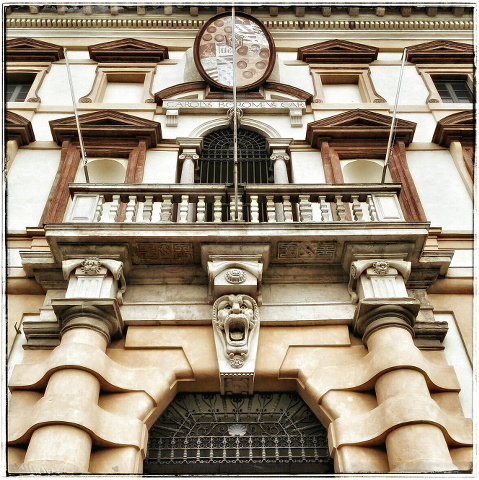
\includegraphics{smallthumb-lesson_I.jpeg}
\setfloatalignment{b}
\end{marginfigure}


\begin{abstract}
\noindent
Queste lezioni riprendono il testo introduttivo al Latino di Pearson\cite{pearson1915}, del quale seguono la numerazione; la struttura di ogni lezione è piuttosto regolare: inizia con \textsc{cenni di morfologia e di sintassi latina}, seguita da un \textsc{piccolo vocabolario} per il lessico; ci sono infine vari \textsc{esercizi} di traduzione e di composizione latina.

\bigskip
\noindent
Lezione VI - Seconda Declinazione: nomi neutri in -um, apposizione, complementi di termine (oggetto indiretto), vocabolario, esercizi.
\end{abstract}

%\printclassoptions

% āēīōū
% ăĕĭŏŭ

\newthought{56. Seconda Declinazione, nomi neutri.} \textbf{dōnum, -ī}, n., \textit{regalo, dono}. Radice \textbf{dōno-}, tema \textbf{dōn-}; \textbf{dōnum grātum}, \textit{regalo gradito}. Radice \textbf{dōno- grāto-}, tema \textbf{dōn- grāt-}. 
\begin{fullwidth}
\begin{table}[!htbp]
  \centering
  \begin{tabular}{l l l l}
    %\toprule
	& \multicolumn{3}{c}{\textsc{Singolare}} \\

    \nom & dōn\textbf{um}, \textit{il dono} (soggetto)    & \hspace{20mm} & dōn\textbf{um} grāt\textbf{um} \\
    \gen & dōn\textbf{ī}, \textit{del dono}   & \hspace{20mm} & dōn\textbf{ī} grāt\textbf{ī} \\
    \dat & dōn\textbf{ō}, \textit{al dono} & \hspace{20mm} & dōn\textbf{ō} grāt\textbf{ō} \\
    \acc & dōn\textbf{um}, \textit{il dono} (compl.oggetto)    & \hspace{20mm} & dōn\textbf{um} grāt\textbf{um} \\
    \voc & dōn\textbf{um}, \textit{o dono}   & \hspace{20mm} & dōn\textbf{um} grāt\textbf{um} \\
    \abl & dōn\textbf{ō}, \textit{per mezzo del dono} & \hspace{20mm} & dōn\textbf{ō} grāt\textbf{ō} \\
	
	\multicolumn{4}{c}{\textemdash} \\
	
	& \multicolumn{3}{c}{\textsc{Plurale}} \\

    \nom & dōn\textbf{a}, \textit{i doni} (soggetto)    & \hspace{20mm} & dōn\textbf{a} grāt\textbf{a} \\
    \gen & dōn\textbf{ōrum}, \textit{dei doni}   & \hspace{20mm} & dōn\textbf{ōrum} grāt\textbf{ōrum} \\
    \dat & dōn\textbf{īs}, \textit{ai doni} & \hspace{20mm} & dōn\textbf{īs} grāt\textbf{īs} \\
    \acc & dōn\textbf{a}, \textit{i doni} (compl.oggetto)    & \hspace{20mm} & dōn\textbf{a} grāt\textbf{a} \\
    \voc & dōn\textbf{a}, \textit{o doni}   & \hspace{20mm} & dōn\textbf{a} grāt\textbf{a} \\
    \abl & dōn\textbf{īs}, \textit{per mezzo dei doni} & \hspace{20mm} & dōn\textbf{īs} grāt\textbf{īs} \\
	
    %\bottomrule
  \end{tabular}
  %\caption[bottom]{Prima Declinazione. \textbf{stella, -ae}, f.}
  \label{tab:normaltab}
  %\zsavepos{pos:normaltab}
\end{table}
\end{fullwidth}

\newthought Osserva come i casi \nom., \acc. e \voc. dei nomi neutri siano uguali, e che al plurale escano in\textbf{-a}. Questo è vero per tutti i nomi neutri di tutte le declinazioni.

\newthought{57. Frasi Modello.} Esamina le seguenti frasi:
\begin{itemize}
\item[\textsc{1.}] \textbf{Marcus agricola filiae equum dat}, \textit{Marco, l'agricoltore, dà a (sua) figlia un cavallo} ovvero \textit{dà un cavallo a (sua) figlia}.  
\item[\textsc{2.}] \textbf{Marcus amico cibum do}, \textit{Do al (mio) amico Marco, del cibo} ovvero \textit{Do del cibo a Marco, amico (mio)}.  
\end{itemize}
Da questi esempi osserviamo che \\
\begin{itemize}
\item[\textsc{1.}] La parola \textbf{agricola} denota la stessa persona di \textbf{Marcus}, e ci dice qualcosa su di essa, ed è declinata nello stesso caso. Una parola così viene detta apposizione. La parola \textbf{Amico} ha la stessa relazione, di apposizione, con \textbf{Marco}.
\item[\textsc{2.}] Le parole \textbf{equum} e \textbf{cibum}, interessate direttamente dall'azione descritta dai rispettivi verbi, sono in caso accusativo; mentre le parole \textbf{filiae} e \textbf{Marco} sono in caso dativo, essendo interessate solo indirettamente dall'azione descritta dal verbo (oggetto indiretto o complemento di termine).
\end{itemize}

\newthought{58. Regole di Sintassi} 
\begin{itemize}
\item[\textsc{1. Apposizione.}] Un'apposizione concorda in \textit{caso} con il nome cui si riferisce (cioè che precisa o limita). 
\item[\textsc{2. Complemento di Termine.}] L'oggetto indiretto di un verbo transitivo (complemento di termine) viene espresso in caso dativo.\sidenote{usato specialmente con verbi che significano dare, fare e dire.}  
\end{itemize}


\newthought{59. Vocabolario} 

\begin{multicols}{2}
    \noindent \hangindent=1em \textbf{bellum, -i}, n., \textit{guerra}.  \\
    \noindent \hangindent=1em \textbf{donum, -i}, n., \textit{regalo, dono}.  \\
    \noindent \hangindent=1em \textbf{oppidum, -i}, n., \textit{città fortificata}.  \\
    \noindent \hangindent=1em \textbf{frumentum, -i}, n., \textit{grano}.  \\
    \noindent \hangindent=1em \textbf{vinum, -i}, n., \textit{vino}.  \\
    \noindent \hangindent=1em \textbf{Marcus, -i}, m., \textit{Marco}.  \\
    \noindent \hangindent=1em \textbf{incola, -ae}, m./f., \textit{abitante}.  \\
    \noindent \hangindent=1em \textbf{Romanus, -i}, m., \textit{romano}.  \\
	
	\noindent \hangindent=1em \textbf{gratus, a, um}, agg., \textit{gradito}.  \\
	\noindent \hangindent=1em \textbf{dō}, v., \textit{io do}.  \\
	\noindent \hangindent=1em \textbf{portō}, v., \textit{io porto}.  \\
	\noindent \hangindent=1em \textbf{in}, prep. con \acc. \marginnote{usato con verbi che significano moto verso qualcosa o qualcuno}, \textit{in, a, contro}; con \abl., \textit{in, su, sopra}  \\
	
\end{multicols}
% āēīōū
% ăĕĭŏŭ

\newthought{60. Esercizi di Ripasso}
\\
\textsc{I.} \quad
\textsc{1.}~Malum servum culpamus. \quad
\textsc{2.}~Laudantne domini superbi servos fidos? \quad
\textsc{3.}~Equi domini sunt in magno horto. \quad
\textsc{4.}~Ubi servi cibum dominorum servant? \quad
\textsc{5.}~Agricolae fidos equos non semper laudant. \quad
\textsc{6.}~Est cibus in domini horto. \quad
\textsc{7.}~Femina amici filiam vocat.
\\
\textsc{II.} \quad
\textsc{1.}~Lei loda il giardino del mio amico. \quad
\textsc{2.}~Un buon cavallo piace a tua figlia. \quad
\textsc{3.}~Il padrone loda l'amico, ma incolpa gli schiavi. \quad
\textsc{4.}~Gli amici dei marinai sono in Grecia. \quad
\textsc{5.}~Perché il giardino piace all'agricoltore? \quad


\newthought{61. Esercizi}
\\
\textsc{I.} \quad
\textsc{1.}~Oppidis; bella; vino. \quad
\textsc{2.}~Marcus nauta est fidus. \quad
\textsc{3.}~Incolis vinum damus. \quad
\textsc{4.}~Bellum Romanis gratum est. \quad
\textsc{5.}~Cibum in oppidum portamus. \quad
\textsc{6.}~Marcus, agricolarum amicus, Romanus est. \quad
\textsc{7.}~Incolae in oppidum frumentum portant. \quad
\textsc{8.}~Filiae reginae in horto sunt. \quad
\textsc{9.}~Vinum Marco nautae dant. \quad
\textsc{10.}~Dona incolis oppidi sunt grata. \quad
\textsc{11.}~Cur vinum servis datis? \quad
\textsc{12.}~Portantne nautae cibum in Galliam?
\\
\textsc{II.} \quad
\textsc{1.}~A Marco, l'agricoltore; per il buon padrone. \quad
\textsc{2.}~Dai ai cavalli del buon grano? \quad
\textsc{3.}~La guerra piace ai fieri romani. \quad
\textsc{4.}~L'agricoltore dà del cibo al cavallo. \quad
\textsc{5.}~La regina dà del vino a MArco, il marinaio. \quad
\textsc{6.}~Portano grano in città. \quad
\textsc{7.}~C'è del buon grano in città.

\newthought{(442.) Lettura e Traduzione.} Un servo fedele.
\\
Lydus est fidus servus agricolae boni in insula. 
Frumentum domini et vinum in oppidum portat, ubi cibus incolis superbis gratus est. 
Malus nauta et amicus in horto sunt. Nauta servum vocat. "Cur vinum, serve, in hortum non portas?" 
Lydus amicis vinum in poculo parvo dat. Nauta vinum bonum laudat sed poculum\sidenote{tazza} parvum et inopiam vini culpat. 
Pugnant. Lydus nautam et amicum superat\sidenote{vince}. Servo pecuniam dant, et Lydus, servus fidus, vinum et frumentum servat.

\begin{figure}[!b]
  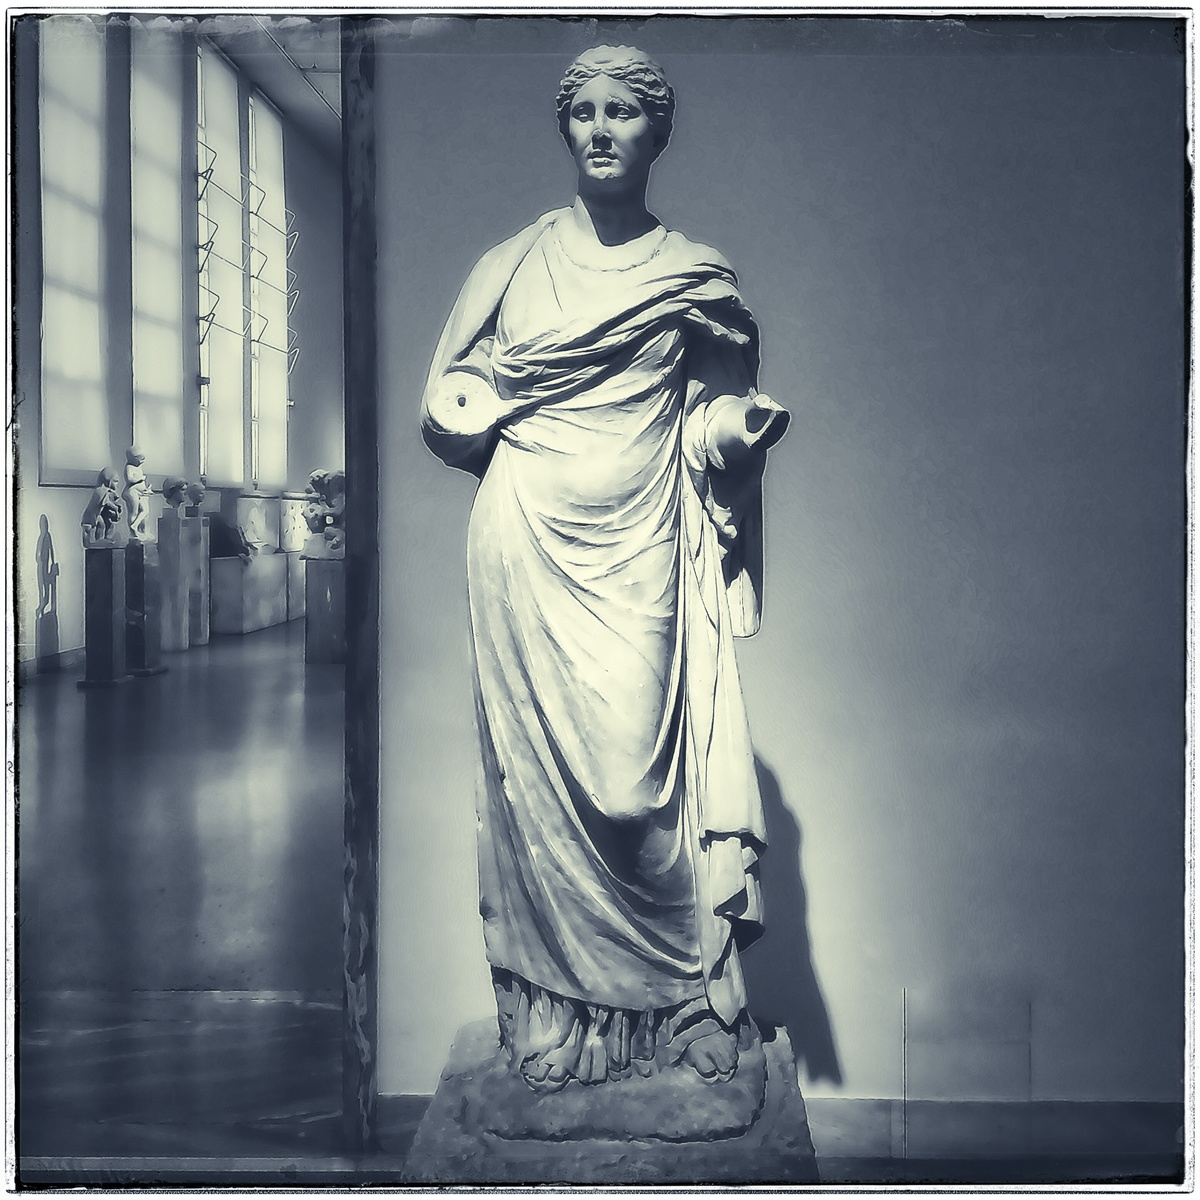
\includegraphics[width=0.8\linewidth]{thumb-lesson_VI.jpeg}
  %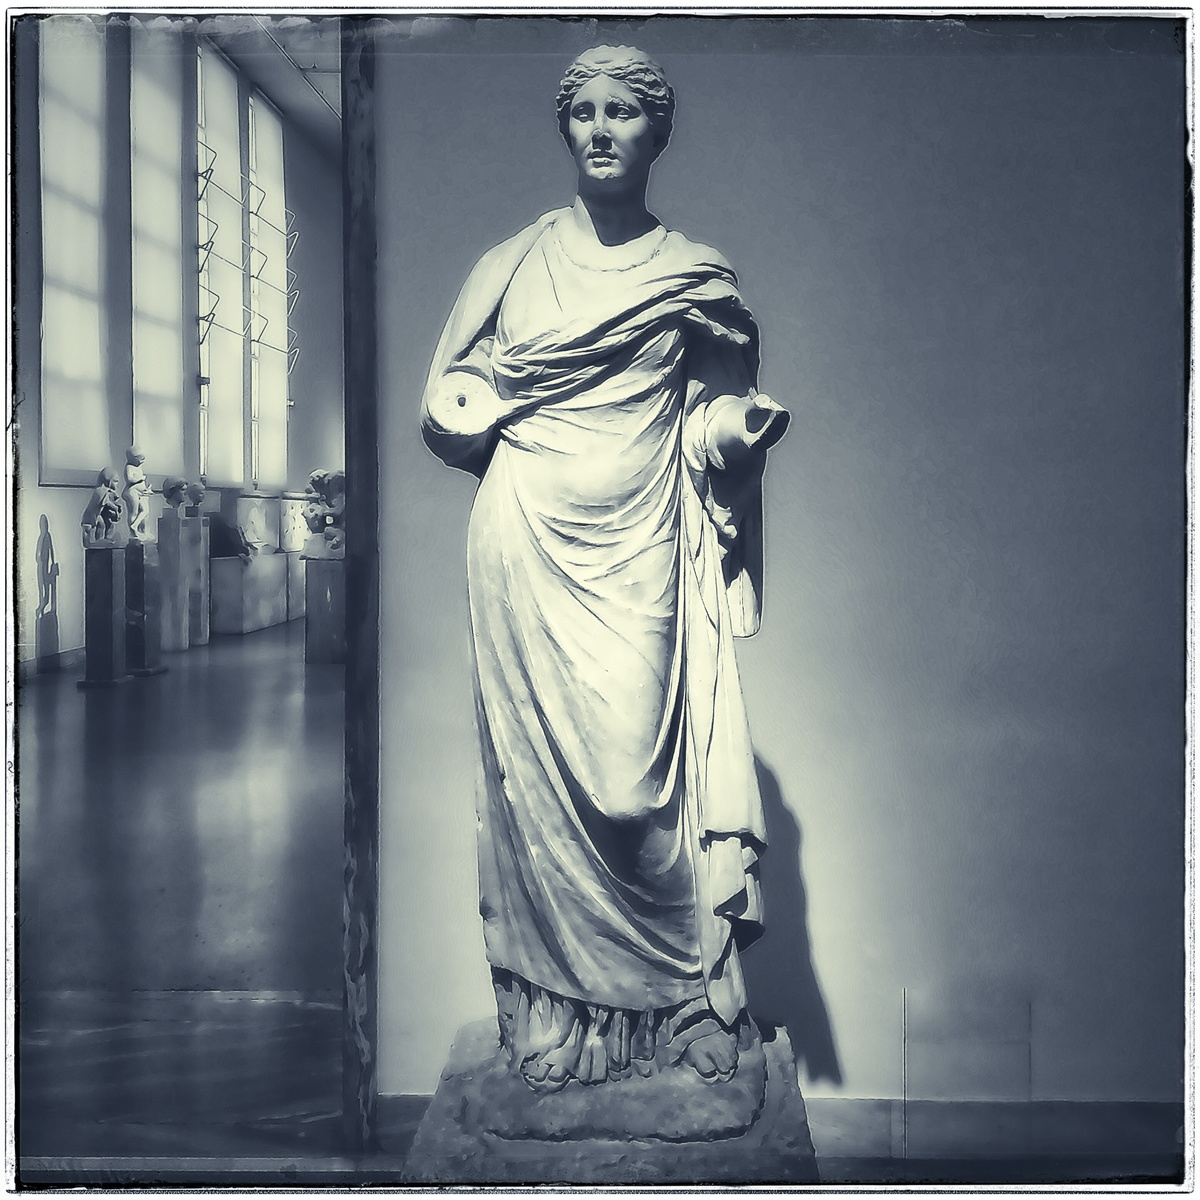
\includegraphics{thumb-lesson_VI.jpeg}
  \caption{Pavia: Almo Collegio Borromeo}
  \label{fig:textfig}
  %\zsavepos{pos:textfig}
  %\setfloatalignment{b}
\end{figure}

 

\nobibliography{latinBiblio}
\bibliographystyle{alpha}


\end{document}
